\chapter{Badania i testy}
\section{Wariancja wyników dla jednej sieci}\label{sec:std_dev}
Ważnym parametrem algorytmu genetycznego jest jego kryterium stopu.
W przypadku eksperymentów opisanych w \ref{sec:levy_test} i \ref{sec:actual_experiment} przyjęto dwa:
\begin{enumerate}
  \item maksymalna liczba iteracji - z przyczyn długiego czasu potrzebenego na obliczenia w przypadku eksperymentu \ref{sec:actual_experiment}, liczbę tę ustalono na 100.
  \item maksymalna liczba iteracji bez poprawy - jeżeli od dłuższego czasu nie obserwujemy poprawy rozwiązania, możemy przyjąć założenie, że znaleźliśmy globalne minimum\label{improvement}
\end{enumerate}
Z punktem \ref{improvement} wiąże się parametr $\epsilon$, który ma sens progu różnicy między nową najlepszą wartością a poprzednią, po przekroczeniu którego możemy mówić o poprawie.

Program eksperymentu został tak zaimplementowany, by reprodukowalność eksperymentu była możliwie najwyższa, tj. by niwelować wpływ generatora pseudolosowego na uzyskane wyniki.
W procesie uczenia sieci neuronowych losowo inicjalizowane są wagi połączeń między neuronami.
Oznacza to, że w przypadku, gdy nie mamym kontroli nad stanem generatora losowego, ta sama w sensie struktury sieć może uzyskać inny wynik po jednej epoce uczenia w zależności od początkowych wag.

W celu minimalizacji wpływu losowego początkowego doboru wag na poprawę wyników sieci, przeprowadzono 100-krotnie uczenie sieci o 4 warstwach, po jednym filtrze w każdej, z różnymi początkowymi wagami.

Następnie wyznaczono wartość średnią (wzór \ref{eqn:mean}) wariancję (wzór \ref{eqn:variance}) zebranych pomiarów.

\begin{equation}\label{eqn:mean}
  \bar{x} = \frac{1}{N} \sum_{i=1}^{N} x_i
\end{equation}

\begin{equation}\label{eqn:variance}
  \sigma^2 = \frac{1}{N} \sum_{i=1}^{N}(x_i - \bar{x})^2
\end{equation}

Dla 100 prób wariancja wyniosła $\sigma^2 =3.708 \times 10^{-6}$, a odchylenie standardowe (pierwiastek kwadratowy z wariancji) $\sigma =1.9255 \times 10^{-3}$.
W związku z tym przyjęto wartość parametru $\epsilon = 4\sigma = 7.702 \times 10^{-3}$, aby wpływ różnej inicjalizacji wag nie był interpretowany przez algorytm genetyczny jako poprawa.

\section{Test działania algorytmu genetycznego}\label{sec:levy_test}
W celu zbadania poprawności działania oraz dostrojenia parametrów algorytmu genetycznego przeprowadzono test szukania minimum funkcji Levego.
Funkcja Levego (\textit{Levy Function}) dana jest wzorem \ref{eqn:levyfunction}:

\begin{equation}\label{eqn:levyfunction}
  f(\mathbf{x}) = sin^2(\pi w_1) + \sum_{i=1}^{d-1} (w_i - 1)^2 [ 1 + 10sin^2(\pi w_i + 1)] + (w_d - 1)^2 [1 + sin^2(2 \pi w_d)]
\end{equation}
gdzie $w_i$ obliczane jest ze wzoru \ref{eqn:wparam}, natomiast d oznacza liczbę wymiarów.
\begin{equation}\label{eqn:wparam}
  w_i = 1 + \frac{x_i - 1}{4}
\end{equation}

Minimum globalne tej funkcji znajduje się w punkcie $ \mathbf{x^*} = (1, ..., 1) $ a jego wartość wynosi zero, tj. $ f(\mathbf{x^*}) = 0 $. \cite{simulationlib}
Wykres tej funkcji dla przypadku 2-wymiarowego przedstawiono na rys. \ref{fig:levyfunction}

\begin{figure}[h!tb]
	 \centering
	 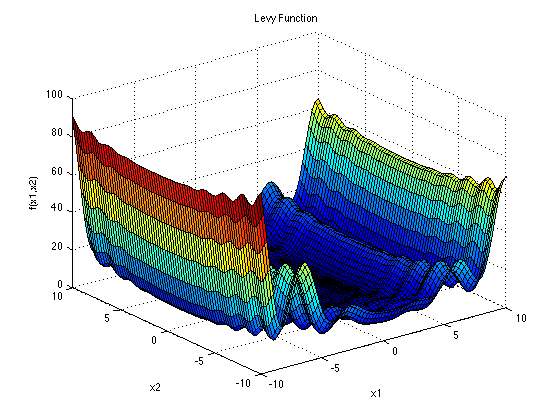
\includegraphics[width = 1.0\linewidth]{img/levy}
	 \caption{Wykres funkcji Levego \\
              Źródło: \cite{simulationlib}}
	 \label{fig:levyfunction}
\end{figure}

Przestrzeń poszukiwań (genotyp osobnika) przyjęto identyczną jak dla problemu optymalizacji struktury konwonlucyjnych sieci neuronowych, tj. $x_i \in \lbrace 1, 2, ... 30, 31 \rbrace$ dla $i = 1..4$.

W celu uniknięcia przypadku, w którym optymalny osobnik powstaje w wyniku mechanizmu naprawiania osbników (opisanego w \ref{sec:individual_fix}) dokonano arbitralnie dobranego przesunięcia wektora $\mathbf{x}$ o wektor $\begin{bmatrix}3 \\ 7 \\ 13 \\ 20\end{bmatrix}$, tak, że optymalne rozwiązanie znalazło się w punkcie $\mathbf{x^*} = \begin{bmatrix}4 \\ 8 \\ 14 \\ 21\end{bmatrix}$.

Jako, że algorytm maksymalizuje funkcję przystosowania osobników, w celu minimalizacji wartości funkcji Levego (funkcji kosztu) została ona zdefiniowana zgodnie ze wzorem \ref{eqn:levy_fitness}. \cite{bialaszewski2012}
\begin{equation}\label{eqn:levy_fitness}
  g(\mathbf{x}) = C_{max} - f(\mathbf{x})
\end{equation}
gdzie $C_{max} = 1000$ w celu spełnienia warunku $g(\textbf{x}) > 0$ dla każdego $\textbf{x}$ w przestrzeni poszukiwań.

Metodą prób i błędów dobrano takie nastawy parametrów algorytmu genetycznego, by znajdował on minimum tej funkcji, tj.
\begin{itemize}
  \item Liczba osobników $N = 100$
  \item prawdopodobieństwo krzyżowania - $p_{c} = 0.9$
  \item prawdopodobieństwo mutacji - $p_{m} = 0.3$
  \item maksymalna liczba iteracji - 100
  \item maksymalna liczba iteracji bez poprawy - 50
  \item liczba najlepszych osobników przechodzących do kolejnego pokolenia - $ N_{k} = 30$
  \item minimalna poprawa $\epsilon = 0.007702$
\end{itemize}

Ostatni parametr dobrany został w sposób opisany w \ref{sec:std_dev}
Operacje genetyczne przeprowadzane są tak jak opisano w \ref{sec:genetic_ops}.
Fenotyp pojedycznego osobnika jest 4-elementową listą liczb całkowitych: $[ x_1, x_2, x_3, x_4]$, natomiast genotyp jest binarną reprezntacją fenotypu na liczbach o długości $m=5$ bitów.
Badanie zostało przeprowadzone dla ziarna generatora ustawionego na wartość 1337.

Na rys. \ref{fig:levy_maxes} i rys. \ref{fig:levy_means} przestawiono odpowiednio maksymalne i średnie (dla całej populacji) wartości funkcji przystosowania w kolejnych iteracjach algorytmu.
Wszystkie kolejne wykresy zostały wykonane przy pomocy biblioteki \textit{Matplotlib}. \cite{Hunter:2007}

\begin{figure}[h!tb]
	 \centering
	 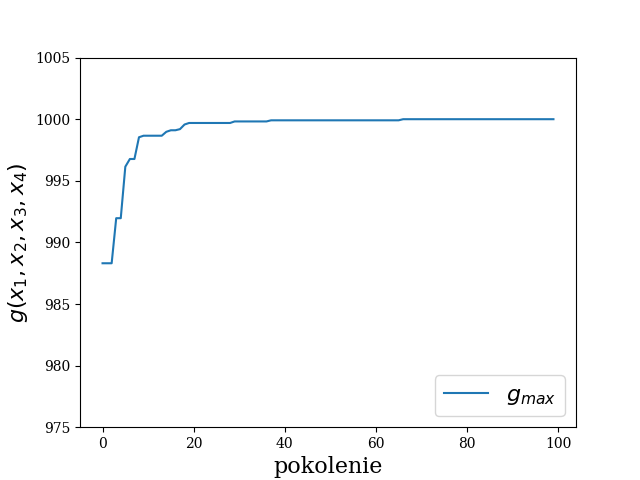
\includegraphics[width = 0.85\linewidth]{img/levy_maxes}
	 \caption{Maksymalne wartości funkcji przystosowania w każdej iteracji dla funkcji Levego \\
              Źródło: praca własna}
	 \label{fig:levy_maxes}
\end{figure}

\begin{figure}[h!tb]
	 \centering
	 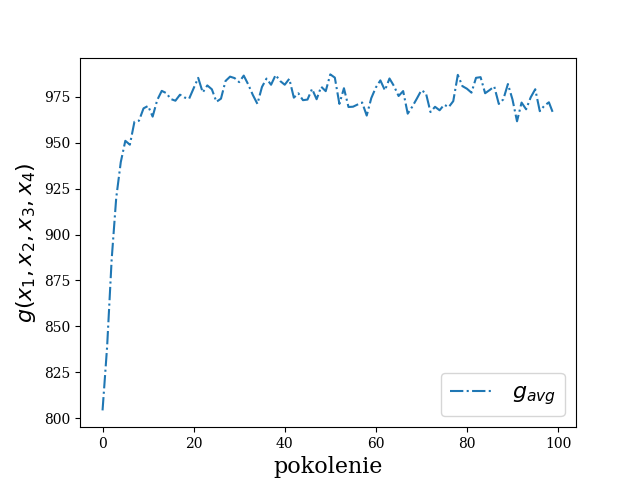
\includegraphics[width = 0.85\linewidth]{img/levy_means}
	 \caption{Średnie wartości funkcji przystosowania w każdej iteracji dla funkcji Levego \\
              Źródło: praca własna}
	 \label{fig:levy_means}
\end{figure}

Zaobserwowane przebiegi wyglądaja jak poprawne przebiegi dla algorytmu genetycznego.
Minimum w punkcie $\mathbf{x^*} = \begin{bmatrix}4 \\ 8 \\ 14 \\ 21\end{bmatrix}$ zostało znalezione w 67. pokoleniu, a kryterium zatrzymania algorytmu, które zadziałało, to maksymalna liczba iteracji równa 100.

Test ten udowodnił, że algorytm genetyczny został zaimplementowany poprawnie i w związku z tym można go w takiej formie wykorzystać do poszukiwania optymalnej struktury konwolucyjnych sieci neuronowych.

\section{Poszukiwanie optymalnej struktury konwolucyjnej sieci neuronowej za pomocą algorytmu genetycznego dla uczenia 1-epokowego}\label{sec:actual_experiment}
Celem tego badania jest sprawdzenie, czy algorytm genetyczny jest w stanie znaleźć optymalną w sensie skutecznośći po jednej epoce uczenia strukturę sieci neuronowej.

Parametry algorytmu genetycznego przyjęto dokładnie takie, do jakich dostrojono algorytm, gdy poszukiwał minimum funkcji Levego, to jest:
\begin{itemize}
  \item Liczba osobników $N = 100$
  \item prawdopodobieństwo krzyżowania - $p_{c} = 0.9$
  \item prawdopodobieństwo mutacji - $p_{m} = 0.3$
  \item maksymalna liczba iteracji - 100
  \item maksymalna liczba iteracji bez poprawy - 50
  \item liczba najlepszych osobników przechodzących do kolejnego pokolenia - $ N_{k} = 30$
  \item minimalna poprawa $\epsilon = 0.007702$
\end{itemize}

\begin{figure}[h!tb]
	 \centering
	 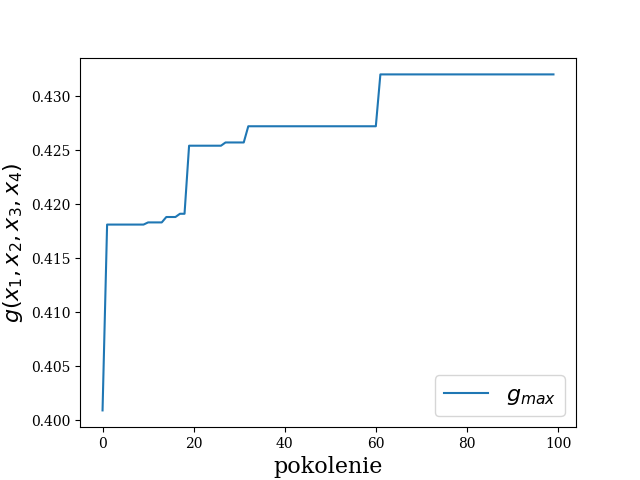
\includegraphics[width = 0.9\linewidth]{img/cnn_maxes_first}
	 \caption{Maksymalne wartości funkcji przystosowania w każdej iteracji dla sieci konwolucyjnych - podejście nr 1\\
              Źródło: praca własna}
	 \label{fig:cnn_maxes_first}
\end{figure}

\begin{figure}[h!tb]
	 \centering
	 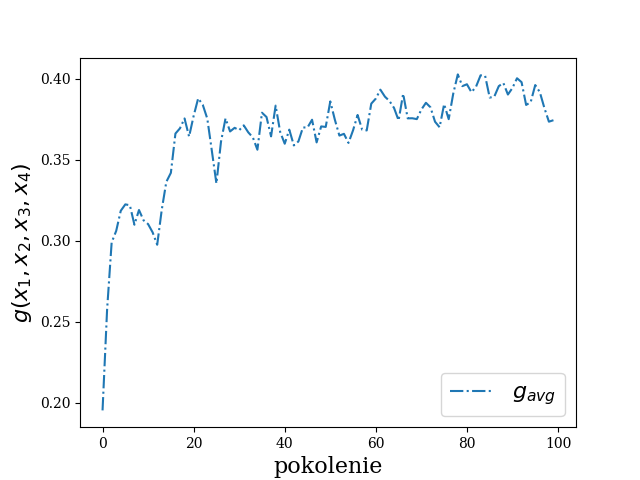
\includegraphics[width = 0.9\linewidth]{img/cnn_means_first}
	 \caption{Średnie wartości funkcji przystosowania w każdej iteracji dla sieci konwolucyjnych - podejście nr 1\\
              Źródło: praca własna}
	 \label{fig:cnn_means_first}
\end{figure}

Przeprowadzono dwa podejścia do tego eksperymentu, z powodu zaobserwowania niepokojących zjawisk w wynikach z podejścia pierwszego.
Na rys. \ref{fig:cnn_maxes_first} i rys. \ref{fig:cnn_means_first} obserwujemy wykresy odpowiednio najwyższych i średnich wartości funkcji przystosowania w populacji.

Badanie zostało przeprowadzone z ziarnem generatora 1337, jednak z przyczyn niezależnych algorytm przerywał działanie i był wzmnawiany odpowiednio w iteracjach 19, 27 i 54, zatem za każdym razem w tych momentach ziarno było ustawiane na 1337.

Przy pierwszym spojrzeniu nie widać nic niepokojącego.
Wykresy przedstawiają poprawne działanie algorytmu genetycznego.
Maksimum funkcji przysotoswania wg. algorytmu znajduje się w punkcie $\mathbf{x^*} = \begin{bmatrix}4 \\ 4 \\ 13 \\ 19\end{bmatrix}$ i zostało odnalezione w 62. iteracji.

Co widoczne będzie dopiero po porównaniu tych wykresów z wykresami na rys. \ref{fig:cnn_maxes} i rys. \ref{fig:cnn_means}, zarówno maksymalne jak i średnie wartości utrzymują się na niższym poziomie.
Jest tak ponieważ pojawiło się nadspodziewanie wiele wartości zbliżonych do 0.1, czego przyczyną może być jedno z następująych dwóch zjawisk:
\begin{enumerate}
  \item sieć ma bardzo złą strukturę (np. 1 filtr konwolucyjny przed warstwą agregującą)
  \item błędy w trakcie uczenia sieci przez węzeł obliczeniowy, które nie powodowały wyłączenia programu, jednak miały istotny wpływ na wynik
\end{enumerate}
Po bliższym przyjrzeniu się kilku przypadkom z danych znaleziono przykłady, w których sieć wygląda, jakby nie miała powodu by osiągać niskie wyniki, np. $\mathbf{x} = \begin{bmatrix}30 \\ 20 \\ 15 \\ 20\end{bmatrix}$, a  jej skutczność klasyfikacji była oceniana na poziomie 10\%.

Przyczyną okazało się złe skonfigurowanie węzłów obliczneniowych.
Wówczas korzystano z węzłów obliczeniowych opartych na obrazie \textit{Data Science Virtual Machine for Linux}.
Obraz ten został wybrany ze względu na preinstalowane biblioteki \textit{Keras, TensorFlow i Numpy}.
Po bliższym przyjrzeniu się sytuacji i ponownym uruchomieniu konkretnego przykładu na maszynie wirtualnej \textit{Data Science Virtual Machine for Linux} ukazało się wiele ostrzeżeń, jak na rys. \ref{fig:warnings}.

\begin{figure}[h!tb]
	 \centering
	 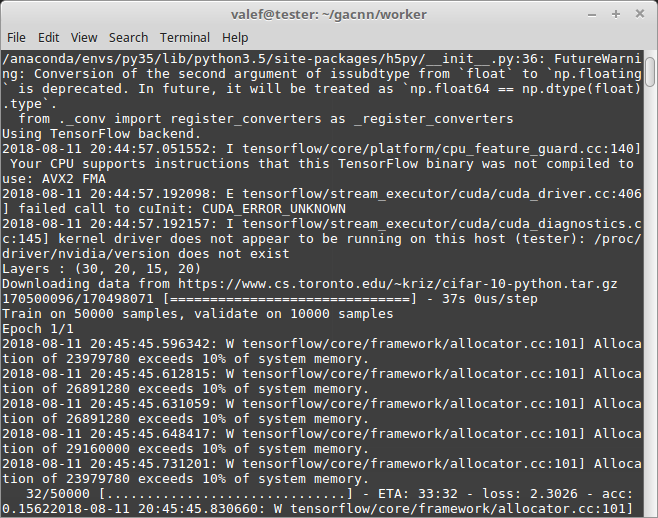
\includegraphics[width = 0.9\linewidth]{img/warnings}
	 \caption{Ostrzeżenia występujące w trakcie pracy węzła obliczeniowego  \\
              Źródło: praca własna}
	 \label{fig:warnings}
\end{figure}

Widać, że maszyna ma problem z alokacją odpowedniej ilości pamięci dla większych sieci, stąd niepoprawne wyniki na poziomie 10\% skuteczności klasyfikacji.
W trakcie pierwszego podejścia przyczynę problemu odnaleziono dopiero po wykonaniu powższych pomiarów.
To podejście okazało się być podejściem testowym i pomogło dopracować system w pełni, tak by działał poprawnie.
Łącznie uczenie wszystkich sieci trwało ok. 24 godzin na 20 węzłach.

Poniżej, na rys. \ref{fig:cnn_maxes} i rys. \ref{fig:cnn_means} przestawiono maksymalne i średnie wartości funkcji przystosowania dla kolejnych generacji w drugim podejściu do eksperymentu.
\begin{figure}[h!tb]
	 \centering
	 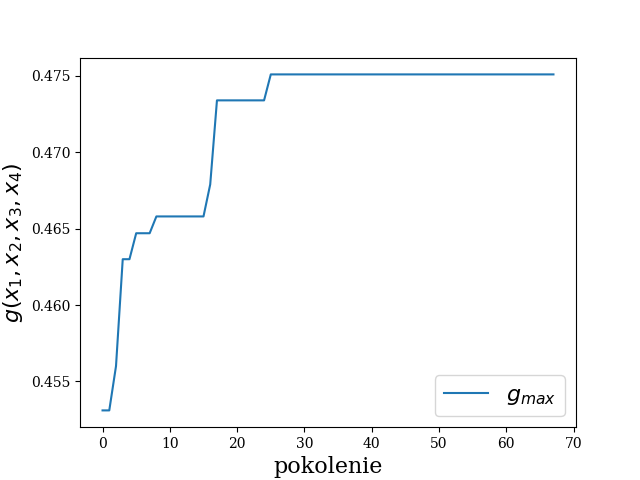
\includegraphics[width = 0.9\linewidth]{img/cnn_maxes}
	 \caption{Maksymalne wartości funkcji przystosowania w każdej iteracji dla sieci konwolucyjnych - podejście nr 2\\
              Źródło: praca własna}
	 \label{fig:cnn_maxes}
\end{figure}

\begin{figure}[h!tb]
	 \centering
	 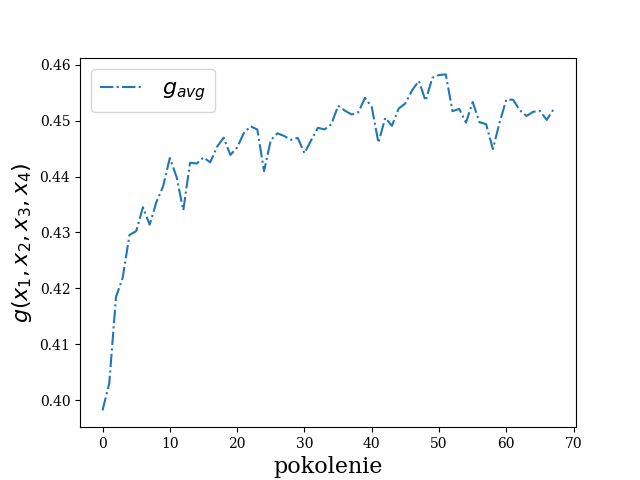
\includegraphics[width = 0.9\linewidth]{img/cnn_means}
	 \caption{Średnie wartości funkcji przystosowania w każdej iteracji dla sieci konwolucyjnych - podejście nr 2\\
              Źródło: praca własna}
	 \label{fig:cnn_means}
\end{figure}

Ponownie jak w teście Levego, wykresy maksymalnych i średnich wartości funkcji przystosowania osobników wyglądają jak typowy dla poprawnie zaimplementowanego algorytmu genetycznego.
Kryterium stopu które zadziałało tym razem to liczba iteracji bez poprawy - 50.
Znalezione przez algorytm rozwiązanie ma postać: $\mathbf{x^*} = \begin{bmatrix}12 \\ 21 \\ 23 \\ 31\end{bmatrix}$ i po jednej epoce uczenia osiąga skuteczność na poziomie 47.51\%.
Niestety, nie jesteśmy w stanie stwierdzić, czy jest to minimum globalne bez wykonywania kosztownego przeszukiwania metodą siłową.

Do drugiego podejścia wymieniono całą infrastukturę węzłów obliczeniowych, tj. zniszczono 20 maszyn wirtualnych opartych na obrazie \textit{Data Science Virtual Machine for Linux} i wymieniono je na obrazy \textit{Ubuntu Server 17.10}, jak opisano w \ref{sec:azure}.
Stwierdzono, że na żadnej z maszyn nie występują ostrzeżenia jak na rys. \ref{fig:warnings}.
Dodatkowo, w stosunku do poprzedniej próby wprowadzono modyfikacje w celu zaoszczędzenia czasu obliczniowego.
Od tego momentu opisany w \ref{sec:queue_system} rozpoczął wewnętrznie sprawdzać, czy powtarzają się osobniki do policzenia, aby nie liczyć ich kilka razy.

Dla drugiego uruchomienia przeprowadzono statystykę ile obliczeń zaoszczędzono.
Sumarycznie nauczono 3827 różnych sieci.
System zliczał liczbę duplikatów w każdej iteracji i przez całe swoje działanie zaoszczędził 501 obliczeń.
W stosunku do pełnej liczby 4328 wyznaczeń funkcji przystosowania uzyskaliśmy 10\% oszczędność czasu.
Dodatkowo, algorytm tym razem nie liczył pełnych 100 iteracji, tylko zakończył swoje działanie w iteracji nr 68 (przy braku poprawy o zadany próg od iteracji nr 18), co ostatecznie zaowocowało ok. 15 h pracy przy drugiej próbie.
Patrząc na wykres \ref{fig:cnn_maxes} widać, że poprawa wyniku pomiędzy 20 i 30 iteracją nie została uwzględniona jako poprawa, gdyż nie przekroczyła zadanego progu $\epsilon$.

\section{Porównanie wyników dla uczenia 1- i 10- epokowego}\label{sec:thesis_proof}
W tym przypadku również przeprowadzono eksperyment dla dwóch przypadków - z infrastukturą opartą na obrazach \textit{Data Science Virtual Machine for Linux} oraz na \textit{Ubuntu Server 17.10}.
Plan eksperymentu przedstawia się następująco:
\begin{enumerate}
  \item Z danych zebranych w badaniu \ref{sec:actual_experiment} wybierz najlepszego, średniego i najsłabszego osobnika w każdej iteracji
  \item Dokonaj uczenia owych osobników przez 10 epok
  \item Dla każdej trójki najlepszy-średni-najgorszy sprawdź, czy kolejność została zachowana
\end{enumerate}

Biorąc pod uwagę, że wszystkich możliwych ustawień trzech osobników jest $P_3 = 3! = 6$, jeżeli nie byłoby żadnego związku pomiędzy wynikiem uzyskanym po 1- a po 10- epokowym uczeniu, stosunek przypadków, w których kolejność została zachowana, do wszystkich przypadków powinien wynieść ok 16\%.

Dla przypadku, tj. węzły obliczeniowe utworzone na podstawie \textit{Data Science Virtual Machine for Linux} - jedynie w 3 przypadkach na 100 kolejność się zgadzała. Wynika to ze złego działania węzłów obliczeniowych - nie jesteśmy w stanie nic powiedzieć, ponieważ zbyt wiele wyników jest zniekształconych w wyniku braku pamięci.
Dla uczenia 10-epokowego jedynie 9 sieci na 156 uczonych uzyskało wynik powyżej 15\% - nie są to osiągi jakie powinna osiągać sieć po 10 epokach uczenia.

Dla przypadku drugiego, tj. infrastuktura oparta o \textit{Ubuntu Server 17.10}, czyli, jak stwierdzono w \ref{sec:actual_experiment} działającej metody obliczania wartości funkcji przystosowania, liczba iteracji dla których kolejność została zachowana wyniosła 40 na 68, co stanowi około 59\%.
Wynik ten jest dużo wyższy niż losowe ustalanie kolejności (poziom 16\%).
Pozwala to wysnuć wniosek, że istnieje pewien związek pomiędzy osiągami sieci po 1-epoce uczenia a ostatecznymi osiągami (tutaj rozumianymi jako 10-epokowe uczenie), gdyż szansa, że trzy sieci zachowają swoją kolejność pod względem jakości klasyfikacji wynosi niemalże 60 \%.

Tutaj również, jak w \ref{sec:actual_experiment} dokonano ulepszenia pomiędzy uruchomieniami algorytmu.
W celu lepszej wizualizacji zachowania sieci w trakcie uczenia, zapisywano historię uczenia, tj. wartości funkcji przystosowania i funkcji kosztu w każdej epoce uczenia uzyskane na zbiorze uczącym oraz uzyskane na zbiorze testowym.
Dzięki temu ulepszeniu można zobaczyć przebieg uczenia dowolnej sieci z arbitralnie wybranej iteracji algorytmu.

\section{Porównanie przebiegu uczenia sieci w pierwszej i ostatniej iteracji algorytmu genetycznego}
Celem tego badania jest sprawdzenie jak zmienia się dynamika uczenia sieci w zależności od jej struktury uzyskanej w wyniku działania algorytmu genetycznego.
Aby zobrazować różnice pomiędzy owymi sieciami zestawiono ze sobą przebiegi uczenia:
\begin{enumerate}
  \item Najlepszej, środkowej i najgorszej sieci z populacji inicjalnej (rys. \ref{fig:iter_learn_first})
  \item J.w. sieci z populacji końcowej (rys. \ref{fig:iter_learn_last})
  \item Najlepszej sieci z pierwszej i ostatniej iteracji algorytmu genetycznego (rys. \ref{fig:iter_learn_best})
\end{enumerate}
Co zaobserwowano:
\begin{itemize}
  \item Wszystkie krzywe uczenia ewolują w ten sam sposób - z każdą epoką uczenia coraz lepiej klasyfikują obrazy
  \item Porównując rys. \ref{fig:iter_learn_first} i rys. \ref{fig:iter_learn_last} widzimy, że w obydwu przypadkach najlepsza i średnia sieć znajdują się blisko siebie, a najgorsza znajduje się stosunkowo daleko pod nimi.
  \item Na rys. \ref{fig:iter_learn_last} widzimy sytuację, w której w dalszych fazach uczenia sieć średnia wyprzedza początkowo najlepszą.
  Zgodnie z \ref{sec:thesis_proof}, do takich sytuacji dochodzi w 40\% iteracji algorytmu.
  Należy przy tym zauważyć, że przecinają się linia średnia z najlepszą, a linia najgorsza pozostaje w bezpiecznej odległości przez kolejne epoki.
  Nasuwa się przy tym wniosek, że im większa początkowa (po jednej epoce) różnica w jakości klasyfikacji obrazów przez sieć, tym większe prawdopodobieństwo, że po pełnym uczeniu relacja pomiędzy jakościami sieci się nie zmieni.
  \item Porównując rys. \ref{fig:iter_learn_first} z rys. \ref{fig:iter_learn_last} lub patrząc na przebiegi na rys. \ref{fig:iter_learn_best} widzimy, że działanie algorytmu genetycznego podnosi pułap, na którym znajdują się krzywe uczenia.
  Wartości zarówno w 1. jak i 10. epoce znajdują się wyżej w iteracji ostatniej niż pierwszej.

\end{itemize}

\begin{figure}[h!tb]
	 \centering
	 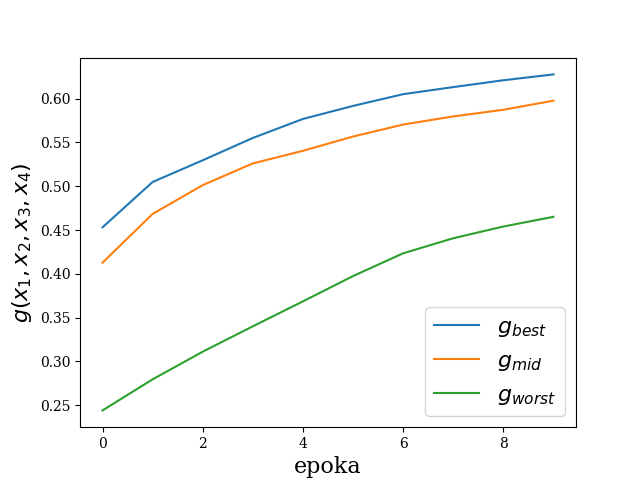
\includegraphics[width = 0.85\linewidth]{img/iter_learn_first}
	 \caption{Przebieg uczenia najlepszej, średniej i najgorszej sieci w pierwszej iteracji algorytmu genetycznego\\
              Źródło: praca własna}
	 \label{fig:iter_learn_first}
\end{figure}

\begin{figure}[h!tb]
	 \centering
	 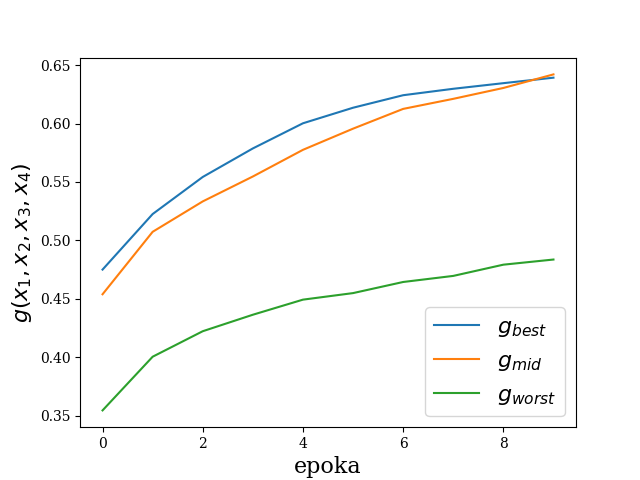
\includegraphics[width = 0.85\linewidth]{img/iter_learn_last}
	 \caption{Przebieg uczenia najlepszej, średniej i najgorszej sieci w ostatniej iteracji algorytmu genetycznego\\
              Źródło: praca własna}
	 \label{fig:iter_learn_last}
\end{figure}

\begin{figure}[h!tb]
	 \centering
	 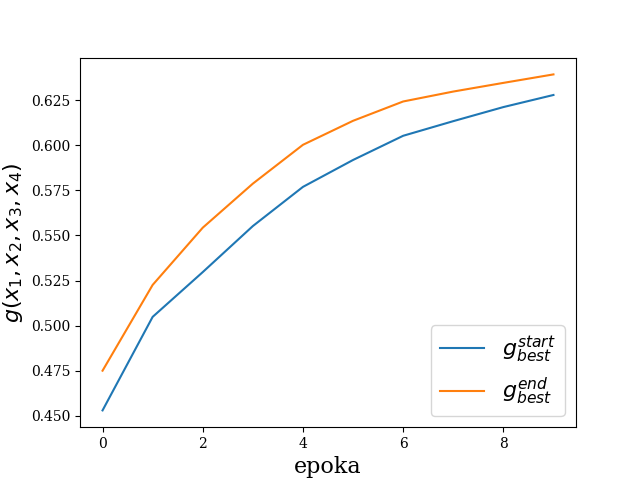
\includegraphics[width = 0.85\linewidth]{img/iter_learn_best}
	 \caption{Przebieg uczenia najlepszej sieci w pierwszej i ostatniej iteracji algorytmu genetycznego\\
              Źródło: praca własna}
	 \label{fig:iter_learn_best}
\end{figure}

Ostatecznie widoczne jest polepszenie procesu uczenia sieci przez algorytm genetyczny.
Nie jest to polepszenie w sensie dynamicznym, gdyż kształt funkcji uczenia prawie się nie zmienia, jednakże w sensie statycznym, czyli wartości na początku i na końcu, widać poprawę.

\section{Osiągi najlepszej według algorytmu sieci po 25 epokach uczenia}
\begin{figure}[h!tb]
	 \centering
	 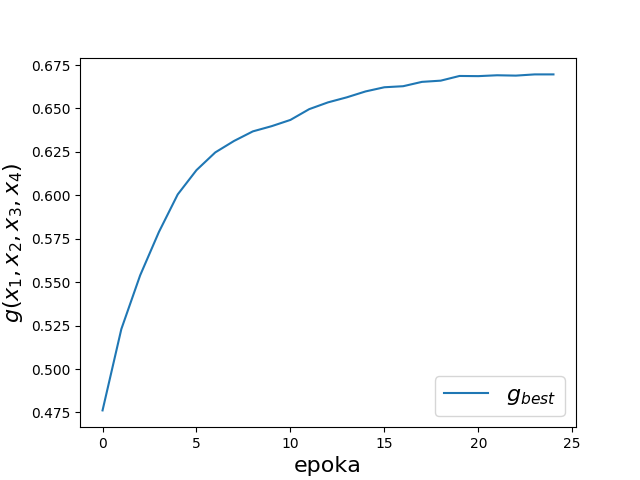
\includegraphics[width = 0.85\linewidth]{img/25epoch}
	 \caption{Przebieg uczenia najlepszego osobnika z \ref{sec:actual_experiment} dla 25 epok\\
              Źródło: praca własna}
	 \label{fig:25epoch}
\end{figure}


Dla rozwiązania $\mathbf{x^*} = \begin{bmatrix}12 \\ 21 \\ 23 \\ 31\end{bmatrix}$ przeprowadzone zostanło uczenie 25-epokowe.
Na rys. \ref{fig:25epoch} przedstawiono krzywą uczenia dla tego przypadku:

Ostateczny wynik uzyskany przez sieć to 67\%.
Jest to gorszy wynik, niż w przykładzie, na którym oparto budowanie modeli sieci i uczenie ich (dostępny pod adresem \url{https://github.com/keras-team/keras/blob/master/examples/cifar10_cnn.py})
Powodem tego może być brak zastosowania warstw \textit{dropout} w sieci modyfikowanej przez algorytm genetyczny, co prowadzi do nadmiernego dopasowania.
Dalsza opytmalizacja powyżej uzyskanych 67\% wymagałaby modyfikacji elementów przyjętych jako stałe w strukturze sieci.
Nie zmienia to faktu, że ów wynik może być najwyższym co można osiągnąć przy tak narzuconej strukturze.
